%%%%%%%%%%%%%%%%%%%%%%%%%%%%%%%%%%%%%%%%%
% Short Sectioned Assignment
% LaTeX Template
% Version 1.0 (5/5/12)
%
% This template has been downloaded from:
% http://www.LaTeXTemplates.com
%
% Original author:
% Frits Wenneker (http://www.howtotex.com)
%
% License:
% CC BY-NC-SA 3.0 (http://creativecommons.org/licenses/by-nc-sa/3.0/)
%
%%%%%%%%%%%%%%%%%%%%%%%%%%%%%%%%%%%%%%%%%

%----------------------------------------------------------------------------------------
%	PACKAGES AND OTHER DOCUMENT CONFIGURATIONS
%----------------------------------------------------------------------------------------

\documentclass[paper=a4, fontsize=11pt]{scrartcl} % A4 paper and 11pt font size
\usepackage[shortlabels]{enumitem}
\usepackage{float}
\usepackage{ctex}
\usepackage{amssymb}
\usepackage{hyperref}
\usepackage{listings}
\usepackage[T1]{fontenc} % Use 8-bit encoding that has 256 glyphs
\usepackage{fourier} % Use the Adobe Utopia font for the document - comment this line to return to the LaTeX default
\usepackage[english]{babel} % English language/hyphenation
\usepackage{amsmath,amsfonts,amsthm} % Math packages

\usepackage{lipsum} % Used for inserting dummy 'Lorem ipsum' text into the template

\usepackage{sectsty} % Allows customizing section commands
%\allsectionsfont{\centering \normalfont\scshape} % Make all sections centered, the default font and small caps
\usepackage{mathrsfs}
\usepackage{fancyhdr} % Custom headers and footers
\usepackage{algorithm}
\usepackage[noend]{algpseudocode}
\algnewcommand\Break{\textbf{break}}

\usepackage{scrextend} % for addmargin
\usepackage{subcaption}
\graphicspath{{p3/}}
%\usepackage{algorithmic}
\usepackage[noend]{algpseudocode}
\usepackage{listings}
\pagestyle{fancyplain} % Makes all pages in the document conform to the custom headers and footers
\fancyhead{} % No page header - if you want one, create it in the same way as the footers below
\fancyfoot[L]{} % Empty left footer
\fancyfoot[C]{} % Empty center footer
\fancyfoot[R]{\thepage} % Page numbering for right footer
\renewcommand{\headrulewidth}{0pt} % Remove header underlines
\renewcommand{\footrulewidth}{0pt} % Remove footer underlines
\setlength{\headheight}{13.6pt} % Customize the height of the header

\numberwithin{equation}{section} % Number equations within sections (i.e. 1.1, 1.2, 2.1, 2.2 instead of 1, 2, 3, 4)
\numberwithin{figure}{section} % Number figures within sections (i.e. 1.1, 1.2, 2.1, 2.2 instead of 1, 2, 3, 4)
\numberwithin{table}{section} % Number tables within sections (i.e. 1.1, 1.2, 2.1, 2.2 instead of 1, 2, 3, 4)

\setlength\parindent{0pt} % Removes all indentation from paragraphs - comment this line for an assignment with lots of text

\newtheorem{theorem}{Theorem}[section]
\newtheorem{corollary}{Corollary}[theorem]
\newtheorem{lemma}[theorem]{Lemma}

%----------------------------------------------------------------------------------------
%	TITLE SECTION
%----------------------------------------------------------------------------------------

\newcommand{\horrule}[1]{\rule{\linewidth}{#1}} % Create horizontal rule command with 1 argument of height

\title{	
\normalfont \normalsize 
%\textsc{university, school or department name} \\ [25pt] % Your university, school and/or department name(s)
\horrule{0.5pt} \\[0.4cm] % Thin top horizontal rule
\huge Analysis and Design of Algorithm - Homework 8\\ % The assignment title
\horrule{2pt} \\[0.5cm] % Thick bottom horizontal rule
}

\author{宁雪妃} % Your name
%\author{Xuefei Ning} % Your name

\date{\normalsize\today} % Today's date or a custom date

\begin{document}

\maketitle % Print the title

%----------------------------------------------------------------------------------------
%	PROBLEM 1
%----------------------------------------------------------------------------------------
\section{Problem 1}
\textbf{22.3-13. 对于有向图$G = (V, E)$来说, 如果$u \leadsto v$意味着图$G$至多包含一条从$u$到$v$的简单路径, 则$G$是单连通图。请给出一个有效算法来判断一个有向图是否是单连通图(singly connected)。}

一个图为单连通图的充分必要条件为, 从图中所有顶点出发的DFS树内都没有cross edge和forward edge。

充分性证明:
\begin{proof}
  证明该命题的逆否命题: 如果$G$不是一个单连通图, 则$G$中必存在从一个顶点出发的DFS树内含有cross edge或者forward edge。

  由于$G$不是一个单连通图, 必定存在$u \in V, v \in V$, $\mbox{s.t. } u, x_1, x_2, \dots, x_n, v$ 和 $u, y_1, y_2, \dots, y_m, v$为两条$u \leadsto v$的简单路径, 且$x_i \neq y_j$(如果$\exists x_i = y_j$, 就可以使$u$或者$v$为$x_i = y_j$, 减小我们的研究范围), 且$x_i$和$y_j$节点之间没连接(如果有连接, 一定可以取新的$u$, $v$找到这两条简单路径)。考虑从$u$开始的深度优先搜索遍历, 当选择了一条路径(不失一般性设为$u, x_1, x_2, \dots, x_n, v$这条路径)往下遍历之后, 在遍历另一条路径时有$y_m \rightarrow v$是一条cross edge。如果特殊情况$m = 0$, 那么$u \rightarrow v$是一条forward edge。所以一定能找到一条cross edge或forward edge。
\end{proof}

必要性证明:
\begin{proof}
  证明该命题的逆否命题: 如果图$G$中的某个DFS存在cross edge或者forward edge, 该图$G$一定不是单连通图。

  若图$G$中的某个DFS存在forward edge $u \rightarrow v$, 说明此时$v$已经为黑色且已经有另一条路径从$u$到达了$v$, 很明显从$u \leadsto v$有至少两条路径。如果某个DFS存在cross edge $u \rightarrow v$, $u$和$v$在这一棵DFS树中的最近共同祖先设为$m$, 那么有在DFS树中$m \leadsto u$加上$u \rightarrow v$, 和$m \leadsto v$这两条从$m$到$v$的简单路径。所以$G$不是单连通图。
\end{proof}

所以只需要对于$V$中每个顶点, 做一遍DFS, 判断是否有DFS树内的forward edge或cross edge, 如果有则返回非单连通图。如果所有顶点开始的DFS树内都没有forward/cross edge, 则为单连通图。复杂度为$O(V (V+E))$。
\\[2ex]

\section{Problem 2}
\textbf{22.5-7. 给定有向图$G = (V, E)$, 如果对于所有节点对$u, v \in V$, 我们有$u \leadsto v$或$v \leadsto u$, 则$G$是半连通的。请给出一个有效的算法来判断图$G$是否是半连通的。证明算法的正确性并分析其运行时间。}

首先易知, 强连通图一定是单连通图, 如果$G$是一个强连通图, 当然也就是一个单连通图。如果$G$不是一个强连通图, 将原图$G$先使用强连通分量计算的算法计算出多个强连通分量$\mathscr{u}_i$, 将每个强连通分量看作一个顶点构成新的$V'$, $E' = \{(\mathscr{u}, \mathscr{v}) | \exists u \in \mathscr{u}, v \in \mathscr{v}. s.t. (u, v) \in E\}$。显然这个强连通分量构成的新图$G' = (V', E')$是一个有向无环图,  这是因为如果$G'$中存在环, 那么这个环连接的几个强连通分量都互相可达, 那么应该属于同一个强连通分量, 矛盾。容易看出判断$G$的单连通性与判断$G'$的单连通性等效。

下面的问题是判断一个有向无环图是否为单连通图, 对于一个有向无环图, 肯定能进行拓扑排序, 在这个排好序的图中, 我们考虑入度为0的点, 也就是拓扑排序DFS过程中结束时间最晚的点, 如果有多于一个入度为0的点。很明显那么这些点之间两个方向都不可达到, 那么$G'$就不是半连通图。如果只有一个入度为0的点$u'$, 那么对于其它任意点$v'$, $u' \leadsto v'$, 所以图$G'$的半连通性在于判断$G'$中去掉$u'$和其发出的边以外剩下的图的半连通性。递推的, 如果这个图为半连通图, 拓扑排序中必存在一条路径经过所有的$G'$中的节点。

算法的伪代码如下:

\begin{algorithm}[H]
  \caption{HALF-CONNECTED($G$)}
  \label{algo:1}
  \begin{algorithmic}
    \State $G' = \mbox{STRONGLY-CONNECTED-COMPONENTS-GRAPH}(G)$ \Comment{得到强连通分量图$G'$}
    \State $\mbox{order} = \mbox{TOPO-SORT}(G')$
    \For{$u=1 \dots G'.V.\mbox{size}-1$}
    \If{$(\mbox{order}[u], \mbox{order}[u+1]) \notin G'.E$}
    \State\Return $\mbox{false}$
    \EndIf
    \EndFor
    \State\Return $\mbox{true}$
  \end{algorithmic}
\end{algorithm}

计算强连通分量需要$O(V+E)$运行时间, 计算拓扑排序需要$O(V+E)$运行时间, 验证是否半连通需要$\Theta(V') = O(V)$时间, 所以一共需要$O(V+E)$的运行时间。

\section{Problem 3}
\textbf{23.2-7. 假定图$G$的一棵最小生成树已经被计算出来。如果在图中加入一个新结点及其相关的新边, 我们需要多少时间来对最小生成树进行更新?}

设加入的新节点为$u$, 相关加入的新边为$E_u = \{e_1, e_2, \dots, e_n\}$, 只需要将$E_u$加入$G$的最小生成树边集$E^{*}$, 在得到的新边集$E' = E^{*} \cup E_u$上做最小生成树算法, 即可得到更新后的最小生成树。这个算法是基于原来不在最小生成树边集$E^{*}$中的边, 在加入新的$E_u$后, 也不可能在新的最小生成树边集$E'^{*}$中。

% 要不要证明..

时间复杂度为$O((V+1+E^{*}+n) \log(V+1)) = O((2V + n)\log(V)) = O((V+n)\log(V))$。

\section{Problem 4}
\textbf{23-1. (次优最小生成树) 设$G = (V, E)$为一连通无向图, 其权重函数为$w: E \rightarrow R$, 假定$|E| \geq |V|$并且所有权重都互相不同。我们定义一棵次优最小生成树如下: 设$\mathscr{T}$为$G$的所有生成树的集合, $T'$为$G$的一棵最小生成树。那么次优最小生成树是生成树$T$, 其满足$w(T) = \min_{T'' \in \mathscr{T} - \{T'\}} {w(T'')}$。}
\begin{enumerate}[a]
\item \textbf{证明: 最小生成树是唯一的, 但次优最小生成树则不一定是唯一的。}

  \begin{proof}
    最小生成树是唯一的: 反设最小生成树不是唯一的, 有两棵树$T_1$, $T_2$均为图$G$的最小生成树。必存在$(u, v) \in T_1$, 且$(u, v) \notin T_2$, 将$(u, v)$加入$T_2$, 必形成一个环, 在这个环中, 设$(x, y)$为环中权重最高的边。如果$(x, y) \neq (u, v)$, 那么$T_2$不是最优的; 如果$(x, y) = (u, v)$, 那么$T_1$不是最优的。

    次优最小生成树不一定是唯一的, 反例如\hyperref[fig:1]{图}所示. 最小生成树为权重为1, 2, 4的边。两棵次小生成树分别为权重为1, 3, 4的边和1, 2, 5的边构成。

  \begin{figure}
    \centering
    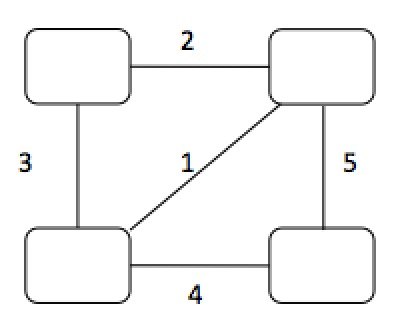
\includegraphics[height=32ex]{1}
    \label{fig:1}
  \end{figure}
  \end{proof}

\item \textbf{设$T$为$G$的一棵最小生成树。证明: 图$G$包含边$(u, v) \in T$和边$(x, y) \notin T$, 使得$T - \{(u, v)\} \cup \{(x, y)\}$是$G$的一棵次优最小生成树。}

  \begin{proof}
设$T'$为图的一棵次小生成树, 令$(u, v) \in T − T'$, 考虑$T' \cup (u, v)$中一定存在一个环, 设环中$(x, y)$为环中全中最高的边。由于$T$为最小生成树, 一定有$(x, y) \neq (u, v)$, 即$w(x, y) > w(u, v)$, 否则就可以用$(x, y)$代替$(u, v)$得到一个权重更小的生成树。那么$w(T' - (x, y) \cup (u, v)) < w(T')$, 所以树$T' - (x, y) \cup (u,v)$为一棵最小生成树, 又最小生成树在权重不一样的无向图中唯一, 命题得证。
  \end{proof}

\item \textbf{设$T$为$G$的一颗最小生成树, 对于任意两个节点$u, v \in V$, 设$\max[u, v]$表示树$T$中从节点$u$到节点$v$的简单路径上的最大权重的边, 请给出一个$O(V^2)$时间复杂度的算法来计算$\max[u, v]$。}

  先生成最小生成树, 需要$O(V^2)$的时间, 然后在最小生成树中从每个点$u$出发做一个DFS遍历, 遍历即可对于其它所有顶点$v$得到$\max[u, v]$, 在最小生成树中的DFS复杂度为$O(V)$。一共$O(V^2)$。

\item \textbf{给出一个有效算法来计算图$G$的次优最小生成树。}

  \begin{enumerate}[1]
  \item 生成图$G$的最小生成树$T$。复杂度为$(O(V^2))$。
  \item 生成$T$中任意一对顶点$u, v$的$\max[u, v]$表格。复杂度为$O(V^2)$。
  \item 对于不在$T$中的边$(u, v)$, 将其加入$T$形成一个环, 在$T$中这个环上全中最大的边$\max[u, v]$可以在上一步的表格中查到。将$\max[u, v]$这条边用$(u, v)$代替, 树的权重增加为$w(u, v) - \max[u, v]$, 找到最小的这个值即可。复杂度为$O(E)$。
  \end{enumerate}

  整个算法的复杂度为$O(V^2 + E) = O(V^2)$。
\end{enumerate}

\end{document}

